\documentclass[aspectratio=169]{beamer}

\usetheme{Madrid}
\usecolortheme{default}

\usepackage{graphicx}
\usepackage{booktabs}
\usepackage{amsmath}
\usepackage{array}
\usepackage[hidelinks]{hyperref}

\graphicspath{{./}{resultImage/}{image/}}

\title[HMM POS Tagger]{Building a Robust Part-of-Speech Tagger using Hidden Markov Model}
\subtitle{Probabilistic Graphical Models Mini Project}
\author[Team 3]{Team 3\\HEAM VISAL}
\institute[ITC]{Institute of Technology of Cambodia\\Department of Applied Mathematics and Statistics}
\date{2025--2026}

\begin{document}

\begin{frame}
  \titlepage
\end{frame}

\begin{frame}{Outline}
  \begin{enumerate}
    \item POS Tagging Problem and Objective
    \item Dataset
    \item HMM Approach
    \item Parameter Estimation
    \item OOV Handling and Log-Space Viterbi
    \item Results and Evaluation
    \item Error Analysis
    \item Conclusion
  \end{enumerate}
\end{frame}

\section{Project Overview}

\begin{frame}{POS Tagging Problem and Objective}
  \begin{itemize}
    \item POS tagging assigns grammar tags to words.
    \item The same word can have different tags.
    \item Example: \emph{watch} is a noun in \emph{my watch is broken}.
    \item Example: \emph{watch} is a verb in \emph{watch the dog}.
    \item Build an HMM POS tagger from scratch and evaluate word-level accuracy.
  \end{itemize}
\end{frame}

\begin{frame}{Dataset}
  \begin{columns}[T]
    \begin{column}{0.46\textwidth}
      \begin{table}
        \centering
        \begin{tabular}{lr}
          \toprule
          \textbf{Item} & \textbf{Value} \\
          \midrule
          Total sentences & 57,340 \\
          Training sentences & 45,872 \\
          Testing sentences & 11,468 \\
          POS tags & 12 \\
          Vocabulary size & 45,153 \\
          \bottomrule
        \end{tabular}
      \end{table}
    \end{column}
    \begin{column}{0.50\textwidth}
      \centering
      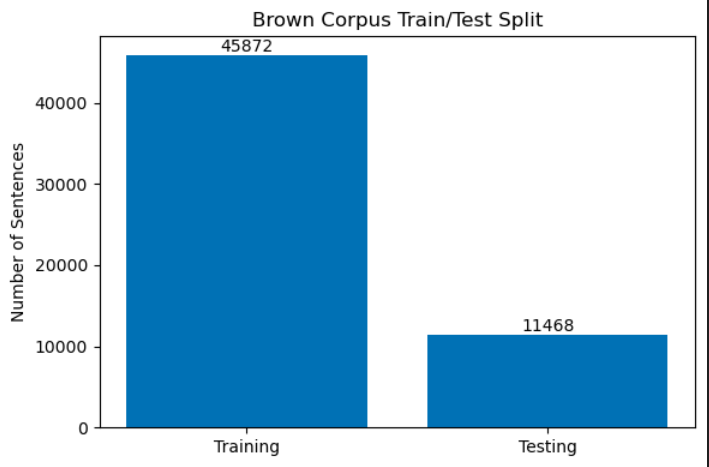
\includegraphics[width=\linewidth]{resultImage/Dataset-split-result.png}
    \end{column}
  \end{columns}
\end{frame}

\section{Methodology}

\begin{frame}{HMM Approach}
  \begin{equation*}
    P(t_1,\ldots,t_n,w_1,\ldots,w_n)
    = \pi(t_1)B_{t_1}(w_1)
    \prod_{i=2}^{n} A_{t_{i-1},t_i}B_{t_i}(w_i)
  \end{equation*}

  \begin{itemize}
    \item Hidden states = POS tags.
    \item Observations = words.
    \item $\pi$ = probability of the first tag.
    \item $A$ = probability of moving from one tag to another.
    \item $B$ = probability of a word given a tag.
  \end{itemize}
\end{frame}

\begin{frame}{Parameter Estimation}
  \begin{itemize}
    \item Estimate $\pi$, $A$, and $B$ from frequency counts.
    \item Use Maximum Likelihood Estimation (MLE).
  \end{itemize}

  \begin{align*}
    \pi(t) &= \frac{\text{Count}(t \text{ starts})}{\text{Total sentences}} \\
    A(i,j) &= \frac{\text{Count}(i \rightarrow j)}{\text{Count}(i)} \\
    B(t,w) &= \frac{\text{Count}(w \text{ emitted by } t)}{\text{Count}(t)}
  \end{align*}
\end{frame}

\begin{frame}{OOV Handling and Log-Space Viterbi}
  \begin{itemize}
    \item OOV problem: unseen words may get zero probability.
    \item Fix: Laplace smoothing with $\alpha = 1.0$ and \texttt{\textless OOV\textgreater}.
    \item Underflow problem: multiplying many small probabilities is unsafe.
    \item Fix: use log-space Viterbi.
    \item Add $\epsilon = 10^{-12}$ before log to avoid $\log(0)$.
  \end{itemize}

  \begin{equation*}
    \log v_t(j) =
    \max_i \left[\log v_{t-1}(i) + \log A(i,j)\right]
    + \log B(j,w_t)
  \end{equation*}
\end{frame}

\section{Results}

\begin{frame}{Results and Evaluation}
  \begin{center}
    \Large\textbf{Accuracy = 93.8\%}
  \end{center}
  \vspace{-0.2cm}
  \begin{columns}[T]
    \begin{column}{0.42\textwidth}
      \begin{table}
        \centering
        \begin{tabular}{lr}
          \toprule
          \textbf{Metric} & \textbf{Value} \\
          \midrule
          Accuracy & 93.8\% \\
          Test words & 232,177 \\
          Correct words & 217,777 \\
          Wrong words & 14,400 \\
          OOV rate & 2.18\% \\
          \bottomrule
        \end{tabular}
      \end{table}
    \end{column}
    \begin{column}{0.54\textwidth}
      \centering
      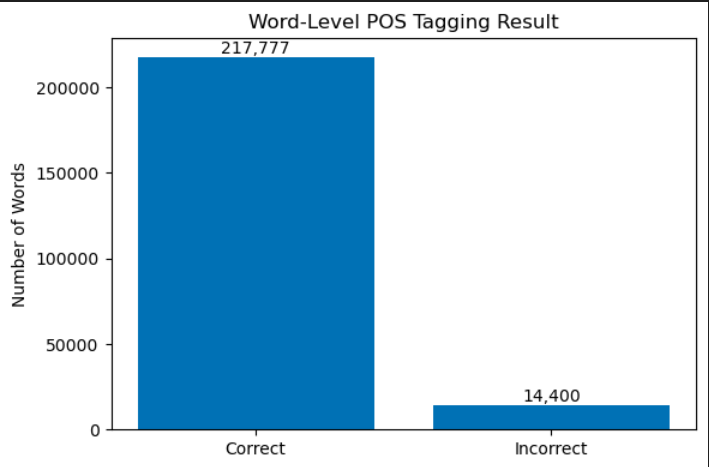
\includegraphics[width=0.94\linewidth]{resultImage/Final-accuracy-result-with-numbers-on-bars.png}
    \end{column}
  \end{columns}
\end{frame}

\section{Error Analysis}

\begin{frame}{Error Analysis}
  \small
  \begin{columns}[T]
    \begin{column}{0.54\textwidth}
      \centering
      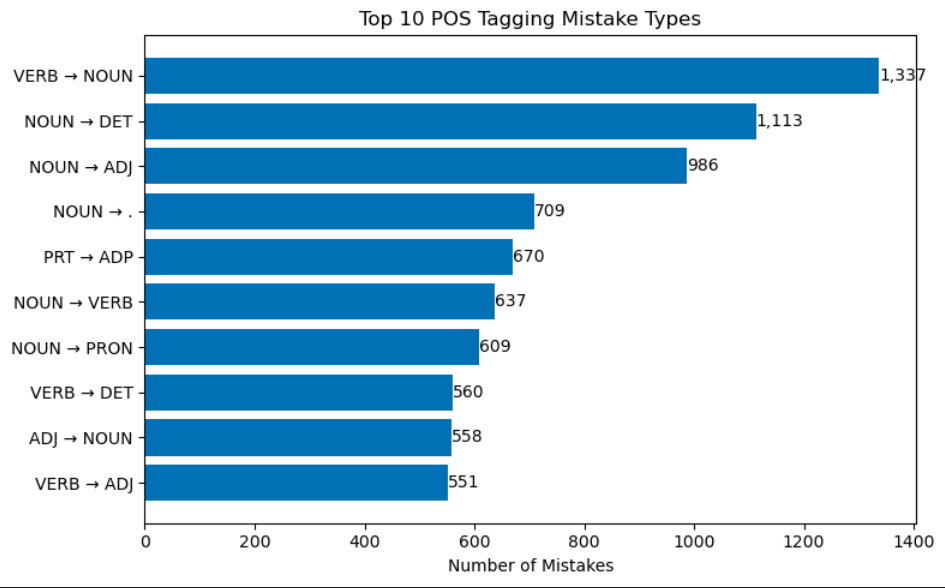
\includegraphics[width=\linewidth]{resultImage/Top-10-mistake-types-with-numbers-on-bars.png}
    \end{column}
    \begin{column}{0.42\textwidth}
      \textbf{Example}

      Sentence: \emph{With tips, the girls average between \$150 and \$200 a week.}

      \vspace{0.1cm}
      \begin{table}
        \centering
        \begin{tabular}{lll}
          \toprule
          \textbf{Word} & \textbf{True} & \textbf{Pred.} \\
          \midrule
          average & VERB & NOUN \\
          \bottomrule
        \end{tabular}
      \end{table}

      \vspace{-0.1cm}
      \textbf{Main causes}
      \begin{itemize}
        \item Ambiguous words.
        \item First-order Markov limitation.
        \item Rare and OOV words.
      \end{itemize}
    \end{column}
  \end{columns}
\end{frame}

\section{Conclusion}

\begin{frame}{Conclusion and Q\&A}
  \begin{itemize}
    \item HMM achieved 93.8\% accuracy.
    \item Laplace smoothing helped with OOV words.
    \item Log-space Viterbi avoided underflow.
    \item Limitations: ambiguity and limited context.
  \end{itemize}

  \vfill
  \centering
  \Large Thank you. Any questions?
\end{frame}

\end{document}
